%\documentstyle[10pt,twoside]{article}
%\documentstyle[twoside]{article}
\documentclass[twoside]{article}
\setlength{\oddsidemargin}{0.25 in}
\setlength{\evensidemargin}{-0.25 in}
\setlength{\topmargin}{-0.6 in}
\setlength{\textwidth}{6.5 in}
\setlength{\textheight}{8.5 in}
\setlength{\headsep}{0.75 in}
\setlength{\parindent}{0 in}
\setlength{\parskip}{0.1 in}

\usepackage{graphicx}
\usepackage{url}
\usepackage{amsmath}
\usepackage{float}

%
% The following commands sets up the lecnum (lecture number)
% counter and make various numbering schemes work relative
% to the lecture number.
%
\newcounter{lecnum}
\renewcommand{\thepage}{\thelecnum-\arabic{page}}
\renewcommand{\thesection}{\thelecnum.\arabic{section}}
\renewcommand{\theequation}{\thelecnum.\arabic{equation}}
\renewcommand{\thefigure}{\thelecnum.\arabic{figure}}
\renewcommand{\thetable}{\thelecnum.\arabic{table}}
\newcommand{\dnl}{\mbox{}\par}

%
% The following macro is used to generate the header.
%
\newcommand{\lecture}[4]{
   \pagestyle{myheadings}
   \thispagestyle{plain}
   \newpage
   \setcounter{lecnum}{#1}
   \setcounter{page}{1}
   \noindent
   \begin{center}
   \framebox{
      \vbox{\vspace{2mm}
    \hbox to 6.28in { {\bf CMPSCI~677~~~Operating Systems
                        \hfill Spring 2018} }
       \vspace{4mm}
       \hbox to 6.28in { {\Large \hfill Lecture #1: #2  \hfill} }
       \vspace{2mm}
       \hbox to 6.28in { {\it Lecturer: #3 \hfill Scribe: #4} }
      \vspace{2mm}}
   }
   \end{center}
   \markboth{Lecture #1: #2}{Lecture #1: #2}
   \vspace*{4mm}
}

%
% Convention for citations is authors' initials followed by the year.
% For example, to cite a paper by Leighton and Maggs you would type
% \cite{LM89}, and to cite a paper by Strassen you would type \cite{S69}.
% (To avoid bibliography problems, for now we redefine the \cite command.)
%
\renewcommand{\cite}[1]{[#1]}

% \input{epsf}

%Use this command for a figure; it puts a figure in wherever you want it.
%usage: \fig{NUMBER}{FIGURE-SIZE}{CAPTION}{FILENAME}
\newcommand{\fig}[4]{
            %\vspace{0.2 in}
            \centerline{\includegraphics[scale=#2]{#4}}
            \begin{center}
            Figure \thelecnum.#1:~#3
            \end{center}
    }

% Use these for theorems, lemmas, proofs, etc.
\newtheorem{theorem}{Theorem}[lecnum]
\newtheorem{lemma}[theorem]{Lemma}
\newtheorem{proposition}[theorem]{Proposition}
\newtheorem{claim}[theorem]{Claim}
\newtheorem{corollary}[theorem]{Corollary}
\newtheorem{definition}[theorem]{Definition}
\newenvironment{proof}{{\bf Proof:}}{\hfill\rule{2mm}{2mm}}

% Some useful equation alignment commands, borrowed from TeX
\makeatletter
\def\eqalign#1{\,\vcenter{\openup\jot\m@th
  \ialign{\strut\hfil$\displaystyle{##}$&$\displaystyle{{}##}$\hfil
      \crcr#1\crcr}}\,}
\def\eqalignno#1{\displ@y \tabskip\@centering
  \halign to\displaywidth{\hfil$\displaystyle{##}$\tabskip\z@skip
    &$\displaystyle{{}##}$\hfil\tabskip\@centering
    &\llap{$##$}\tabskip\z@skip\crcr
    #1\crcr}}
\def\leqalignno#1{\displ@y \tabskip\@centering
  \halign to\displaywidth{\hfil$\displaystyle{##}$\tabskip\z@skip
    &$\displaystyle{{}##}$\hfil\tabskip\@centering
    &\kern-\displaywidth\rlap{$##$}\tabskip\displaywidth\crcr
    #1\crcr}}
\makeatother

% **** IF YOU WANT TO DEFINE ADDITIONAL MACROS FOR YOURSELF, PUT THEM HERE:



% Some general latex examples and examples making use of the
% macros follow.

\begin{document}

%FILL IN THE RIGHT INFO.
%\lecture{**LECTURE-NUMBER**}{**DATE**}{**LECTURER**}{**SCRIBE**}
\lecture{13}{March 19}{Prashant Shenoy}{\textbf{Pegah Taheri}}

\section{Logical Clocks}
In many scenarios in a distributed systems we want to know the ordering of some events instead of the actual time that an event has occurred. For these scenarios we can use a "logical clock", which won't need clock synchronization and would give us time stamps of the events instead of their actual time.\newline
If two machines are not interacting with each other, we assume they are not part of the same system and there is no need to sync them, but on the machines that are part of the same system, processes should agree on the ordering.
\section{Event ordering}
We want to define a total ordering for events that occur on different machines in one system, so if we look at the timeline we can say which event happened first. We make some assumptions
\begin{enumerate}
    \item Events in one single machine is always naturally ordered.
    \item Across processes on the same machine it is still very straight forward to order events based on their actual time.
    \item But in a distributed system, we can't have a global clock. A global clock is a perfectly synchronized clock across all machines. But even with clock synchronization there is going to be some error of getting a global clock.
    % \item Local clocks could be out of order and unsynchronized.
\end{enumerate}
We use the Lamport technique, based on the idea that processes are exchanging messages and message exchanging is a naturally ordered event where a message is not received before it was sent.\newline
So we can use the two events of sending a message and receiving messages to order events across processes.\newline
If we have two processes A and B across machines with their own timelines, and machine A is sending a message to machine, in each machine's single process we know the order. Now, given that we always know that send happens before a receive, we know all of the events that precedes a send, has happened before the receive and all of the events after the receive have happened after the message was sent (Figure :\ref{fig:figure_of_send_receive}).\newline
\begin{figure}[h]
\centering
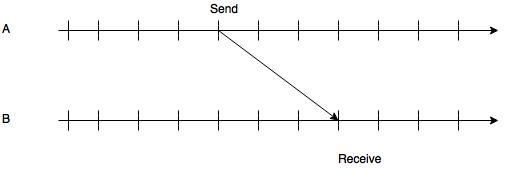
\includegraphics[width=400]{diagram1.jpg}
\label{fig:figure_of_send_receive}
\caption{}
\end{figure}
\subsection{Goal}
So the goal is to order events using the fact that if A precedes B, then the clocktime of A should be before B

$\text{If A}\rightarrow\text{B, then C(A) \textless}\text{ C(B)}$

(If A and B are concurrent, then C(A) \textless, =, or \textgreater C(B))

\subsection{Algorithm}
Logical clocks can be implemented essentially with an integer associated with each machine/process. Each processor will have a logical clock $LC_i$ and every time a local event occurs, the integer is incremented. The local events are defined in the application based on what is cared about. When processes exchange messages, then piggyback the local clock from the sending process to the receiving process. This guarantees a partial ordering of events, since obviously a message must be sent before it is received.

-Each processor maintains a logical clock LC\textsubscript{i}

-Whenever event occurs locally at I, LC\textsubscript{i} = LC\textsubscript{i} + 1

-When i sends message to j, piggyback LC\textsubscript{i}

-When j receives messages from i, if LC\textsubscript{j} \textless \text{ LC\textsubscript{i}} then LC\textsubscript{j} = LC\textsubscript{i} + 1 else do nothing
So in the above example, the receiver receives a message with time stamp 4 while the receiver's event time stamp states 3. Here it takes the $max(3,4)+1$ as its time stamp.
\begin{figure}[h]
\centering
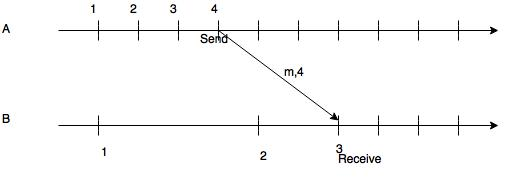
\includegraphics[width=\textwidth]{diagram_2.jpg}
\label{fig:piggy back clock}
\caption{}
\end{figure}
In the example below (Figure:\ref{fig:book_slide_example}), in part a the Lamport algorithm is not used and the receiver's timestamps are not adjusted. In part b, they are adjusted to ensure that the relationship is maintained.
\begin{figure}[h]
\centering
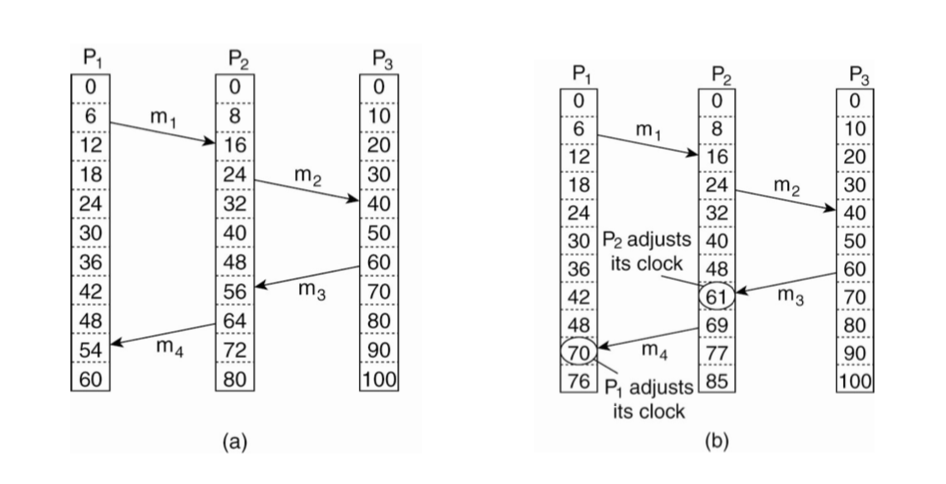
\includegraphics[width=\textwidth]{diagram3.jpg}
\label{fig:book_slide_example}
\caption{}
\end{figure}
This method of ordering is a partial ordering, which by looking at the time stamp we can tell that we can not compare the actual time of the events just by comparing the time stamps.
\section{Total Order}
To arbitrary impose an ordering, the clock value is changed to a decimal value and  the process id of each process (which has its own clock) is appended to the process's clock value with a "." suffix. Because we are using the Lamport's clock, for anything that is not comparable we use the process id to compare them. 

\section{Causality}
In Lamport's algorithm we couldn't say that if the clock value of A is less than B, then A has happened before B. We want this relationship to also be true for the clock values. So we have to determine a causal relationship between events in a distributed system. If the clocktime of A is before B then A should have also preceded B, so the time stamps are comparable and meaningful.

If C(A) \textless C(B) then A \textless B


\section{Vector Clocks}
\begin{itemize}
    
\item Instead of just one Integer, every process maintains a vector as long as the number of processes. So each process $i$ has a vector V that $V_i[i]$ shows the clock of $i_{th}$ logical clock and $V_i[j]$ shows that for the $j_{th}$ process.

\item Update vector clocks as follows
\begin{itemize}
    \item Local event: increment $V_i[I]$
    \item Send a message :piggyback entire vector V
    \item Receipt of a message: $V_j[k] = \max( V_j[k],V_i[k])$
    \item Receiver is told about how many events the sender knows occurred at another process k 
\item Also $V_j[i] = V_j[i]+1$
\end{itemize}


\end{itemize}

\begin{figure}[H]
    \centering
    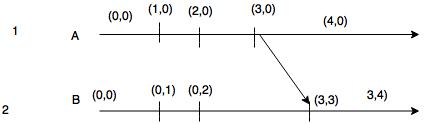
\includegraphics{diagram4.jpg}
    \caption{Vector clocks}
    \label{fig:vector clocks}
\end{figure}
Vector clocks are used to determine causal relationships. It can guarantee the reverse of what logical clocks guarantee. 
\subsection{Example: Totally-Ordered Multicasting}

We assume two users are making updates on their accounts. Because these are replicated DBs used here, queries should be made to both replicas. Now it is important from a consistency perspective that all the updates are made at the same order. Otherwise there might have a situation that two replicas with different ordered queries performed on them might be a problem. If the two users are unrelated there won't be a problem because the queries are unrelated but if users are actually modifying related records there will be a problem that leads to inconsistency. 

Here we can use a total ordering solution.


\subsection{Algorithm}
Take lamport's, and add multicast to get total ordering

-If send(m) $\rightarrow\text{ send(n) }\Rightarrow\text{ deliver(m) }\rightarrow\text{ deliver(n)}$

-Each process i maintains a vector V\textsubscript{i}

-V\textsubscript{i}[i] number of events that occurred at i

-V\textsubscript{i}[j] number of events process i knows have occurred at process j

-Update vector clock:

-Local event: increment i\textsuperscript{th} element of vector. V\textsubscript{i}[i] = V\textsubscript{i}[i] + 1

-Send a message: piggyback entire vector V

-Receipt of a message: V\textsubscript{j}[k] = max(V\textsubscript{j}[k], V\textsubscript{i}[k])
\section{Global state}
Problem definition: We want to run a distributed application and one of n processes crashes. We can either kill all of them and restart, or we can take snap shots of the distributed application so we can go to the latest snap shot, instead of all the way to the beginning, and restart. To do that, we have to define the notion of global state which is the local state of every process as well as all the processes that are in transit (messages that are sent). 
\section{Distributed Snapshots}
A simple technique to capture that is to assume a global synchronized clock and freeze all machines at the same time and capture whatever that are in all memories at the exactly same time and capture everything that is in transit.

But there is no global clock synchronization. Distributed snapshotting is a mechanism that gives a consistent global state.

Things needed in checkpoint are the local state of each process, each message sent in process, state of the queues, and all outstanding messages.

State snapshots can be visualized as horizontal time lines with a line intersecting them at snapshot time. Everything to the left is the past and everything to the right is the future of the snap shot. This makes it easy to spot consistency in cuts. Consistent cuts happen when send/receive processes happen checkpoint either before or after message complete, or a message is sent in past and received in future.

Inconsistent cuts happen when process checkpoints after message complete while others checkpoint before. This can result in messages being sent more than once if restarted. A receive of a message can not be in the past of the snap shot cut while the sending of it is in future.

\subsection{Goal (via photography example):}
Photographer taking a picture of the sky with birds flying around in it. Can't capture entire sky in one pic. Stitch pics of left, middle, right parts of sky. If you take a picture of the left, and then take a picture of the middle, but a bird has flown from left to the middle, you have taken a picture of that bird twice because of inconsistency. The goal is to get a consistent photo - for it to be consistent, then all three pictures have captured all the birds that were in the sky.

\end{document}
